%%%%%%%%%%%%%%%%%%%%%%%%%%%%%%%%%%%%%%%%%
% Beamer Presentation
% LaTeX Template
% Version 1.0 (10/11/12)
%
% This template has been downloaded from:
% http://www.LaTeXTemplates.com
%
% License:
% CC BY-NC-SA 3.0 (http://creativecommons.org/licenses/by-nc-sa/3.0/)
%
%%%%%%%%%%%%%%%%%%%%%%%%%%%%%%%%%%%%%%%%%

%----------------------------------------------------------------------------------------
%	PACKAGES AND THEMES
%----------------------------------------------------------------------------------------

\documentclass{beamer}

\mode<presentation> {
	
	% The Beamer class comes with a number of default slide themes
	% which change the colors and layouts of slides. Below this is a list
	% of all the themes, uncomment each in turn to see what they look like.
	
	\usetheme{default}
	%\usetheme{AnnArbor}
	%\usetheme{Antibes}
	%\usetheme{Bergen}
	%\usetheme{Berkeley}
	%\usetheme{Berlin}
	%\usetheme{Boadilla}
	%\usetheme{CambridgeUS}
	%\usetheme{Copenhagen}
	%\usetheme{Darmstadt}
	%\usetheme{Dresden}
	%\usetheme{Frankfurt}
	%\usetheme{Goettingen}
	%\usetheme{Hannover}
	%\usetheme{Ilmenau}
	%\usetheme{JuanLesPins}
	%\usetheme{Luebeck}
	%\usetheme{Madrid}
	%\usetheme{Malmoe}
	%\usetheme{Marburg}
	%\usetheme{Montpellier}
	%\usetheme{PaloAlto}
	%\usetheme{Pittsburgh}
	%\usetheme{Rochester}
	%\usetheme{Singapore}
	%\usetheme{Szeged}
	%\usetheme{Warsaw}
	
	% As well as themes, the Beamer class has a number of color themes
	% for any slide theme. Uncomment each of these in turn to see how it
	% changes the colors of your current slide theme.
	
	%\usecolortheme{albatross}
	\usecolortheme{beaver}
	%\usecolortheme{beetle}
	%\usecolortheme{crane}
	%\usecolortheme{dolphin}
	%\usecolortheme{dove}
	%\usecolortheme{fly}
	%\usecolortheme{lily}
	%\usecolortheme{orchid}
	%\usecolortheme{rose}
	%\usecolortheme{seagull}
	%\usecolortheme{seahorse}
	%\usecolortheme{whale}
	%\usecolortheme{wolverine}
	
	%\setbeamertemplate{footline} % To remove the footer line in all slides uncomment this line
	%\setbeamertemplate{footline}[page number] % To replace the footer line in all slides with a simple slide count uncomment this line
	
	%\setbeamertemplate{navigation symbols}{} % To remove the navigation symbols from the bottom of all slides uncomment this line
}

\usepackage{sidecap}%[capbesideposition=inside, facing=yes,capbesidesep=quad]
\usepackage{graphicx} % Allows including images
\usepackage{booktabs} % Allows the use of \toprule, \midrule and \bottomrule in tables
%----------------------------------------------------------------------------------------
%	TITLE PAGE
%----------------------------------------------------------------------------------------

\title[Four Models]{Four Models for Severe Weather Deaths} % The short title appears at the bottom of every slide, the full title is only on the title page

\author{Jason Michaels (jam521), Niko Paulson (ndp32), \\Miranda Seitz-McLeese (mgs85) } % Your name
%\institute[UCLA] % Your institution as it will appear on the bottom of every slide, may be shorthand to save space
%{
%	University of California \\ % Your institution for the title page
%	\medskip
%	\textit{john@smith.com} % Your email address
%}
\date{May 11, 2017} % Date, can be changed to a custom date

\begin{document}

	\begin{frame}
		\titlepage % Print the title page as the first slide
	\end{frame}
	
	\begin{frame}
		\frametitle{Overview} % Table of contents slide, comment this block out to remove it
		\tableofcontents % Throughout your presentation, if you choose to use \section{} and \subsection{} commands, these will automatically be printed on this slide as an overview of your presentation
	\end{frame}
	
	%----------------------------------------------------------------------------------------
	%	PRESENTATION SLIDES
	%----------------------------------------------------------------------------------------
	\section{Introduction} 
	\begin{frame}
		\frametitle{Introduction: Goals and Motivation}
		Understanding how and at what rate severe weather events become lethal in the United States has tremendous health impacts. Understanding the distribution of death counts can help meteorologists better predict outcomes.
	\end{frame}
	\begin{frame}
		\frametitle{Introduction: Data}
		The data for this project was taken from the NOAA severe weather events dataset. 
		In its original form this dataset includes a variety of measurements for all forms of severe weather in the United States dating from 1950. In the interest of time we restricted the dataset to:
		\begin{itemize}
			\item Deaths directly attributable to Tornadoes and Flash floods 
			\item Occurred between 1996-2016
		\end{itemize}
	\end{frame}
	\begin{frame}
		\frametitle{Introduction: Zero Inflated Models}
			Fortunately, the vast majority of severe weather events in the United States involve no deaths, therefore we wanted to also account for the possibility of structural zeros, therefore we also considered zero inflated variants. A zero inflated model is a combination of the original distribution and a point mass at zero. If the original distribution is $p(x)$ then $$z(x) = \begin{cases}
			\sigma + (1-\sigma)*p(0) &x=0\\
			(1-\sigma)*p(x) &x\ne0
			\end{cases}$$
	\end{frame}
	\begin{frame}
		\frametitle{Introduction: Four Models}
				In this paper we compare four possible models for the deaths: 
				\begin{enumerate}
					\item Poisson
					\item Negative Binomial
					\item Zero Inflated Poisson
					\item Zero Inflated Negative Binomial
				\end{enumerate}
	\end{frame}
	
	\section{Poisson Model}
	\begin{frame}
		\frametitle{Poisson Model}
		% Slide one
		The Poisson model has one parameter, $\lambda$ that represents the expected number of occurrences of the event of interest. For a single random variable $x$, the probability density is:
$$p(x|\lambda)=\frac{\lambda^xe^{-\lambda}}{x!}.$$
	\end{frame}
	\begin{frame}
		\frametitle{Poisson Model}
		% Slide two
		The Poisson likelihood can be written as follows:
$$\mathcal{L}(X|\lambda)\propto\lambda^{n\bar{X}}e^{-n\lambda}.$$  Since we want the data to speak for itself we use Jeffreys' prior, $$\pi(\lambda)\propto\lambda^{1/2-1}e^{-0\cdot\lambda}.$$ Thus the posterior is: $$p(\lambda|X)=\lambda^{n\bar{X}+1/2-1}e^{-n\lambda}.$$
We recognize this as the kernel of a gamma distribution, namely
$$\lambda|X\sim\mathcal{G}amma(n\bar{X}+1/2,n).$$

	\end{frame}
	\begin{frame}
		\frametitle{Poisson Model}
		% Slide three
		\begin{table}
    \centering
    \caption{Posterior distributions of $\lambda$, for both event types. From 10,000 samples for each variable we obtained the following values: the second column is the median of the sample for $\lambda$, with the 95 percent credible interval in parentheses.}
    \label{t:rPOIS}
    \begin{tabular}{| l | l | l |}
    \hline
    Event Type & $\lambda$  \\ \hline
    Tornado & 0.0592 (0.0564, 0.0620) \\ \hline
    Flash Flood & 0.0179 (0.0170, 0.0189) \\ \hline
    \end{tabular}
\end{table}
	\end{frame}	
		\begin{frame}
		\frametitle{Poisson Model}
		% Slide four
		\begin{figure}[p]
\centering
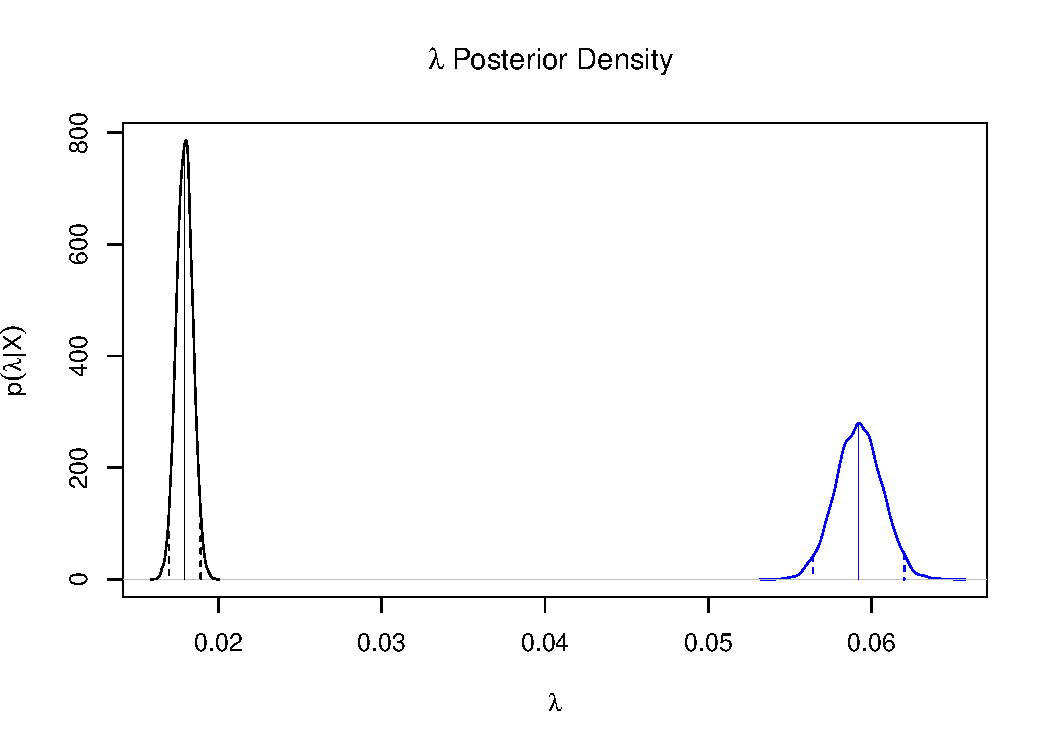
\includegraphics[width=.65\textwidth]{figure/POIS_Density.pdf}
\caption{Posterior density plots (Poisson model) for flood parameters (in blue), and tornado parameters (black). The solid line represents the median and the dashed lines indicate the 95\% confidence interval.}
\label{f:poisdensity}
\end{figure}
	\end{frame}
	
	\section{Negative Binomial Model}
	\begin{frame}
		\frametitle{Negative Binomial}
		% Slide one
		The Negative Binomial model has two parameters, $r,p$, we are mostly interested in $p$. For a single random variable $x$, the probability density is:
$$p(X|r,p)=\frac{\Gamma(r+x)}{\Gamma(r)x!}p^{x}(1-p)^{r}.$$
	\end{frame}
	\begin{frame}
		\frametitle{Negative Binomial}
		% Slide two
		The likelihood of the Negative Binomial can be written as:
$$\mathcal{L}(X|r,p)=\Bigg[\prod_{i=1}^n\frac{\Gamma(r+x_i)}{\Gamma(r)x_i!}\Bigg]p^{n\bar{X}}(1-p)^{nr}.$$
Since we want the data to speak for itself, we will use Jeffreys' prior. For the Negative Binomial distribution this is:
$$\pi(r,p)=r^{1/2}p^{-1}(1-2)^{-1/2}.$$
We are interested in the conditional posterior of $p|r,X$ given by:
$$p(p|r,X)\propto p^{n\bar{x}-1}(1-p)^{nr+1/2-1}$$ 
This is the kernel of a beta distribution, namely
$$p|r,X\sim\mathcal{B}eta(n\bar{X},nr+1/2).$$
	\end{frame}
		\begin{frame}
		\frametitle{Negative Binomial}
		% Slide three
		\begin{table}
    \centering
    \caption{Posterior distributions of $p$, for both event types. From 10,000 samples for each variable we obtained the following values: the second column is the median of the sample for $p$, with the 95 percent credible interval in parentheses.}
    \label{t:rNB}
    \begin{tabular}{| l | l | l |}
    \hline
    Event Type & $p$  \\ \hline
    Tornado & 0.0559 (0.0534, 0.0585) \\ \hline
    Flash Flood & 0.0176 (0.0167, 0.0186) \\ \hline
    \end{tabular}
\end{table}
	\end{frame}
		\begin{frame}
		\frametitle{Negative Binomial}
		% Slide four
		\begin{figure}[p]
\centering
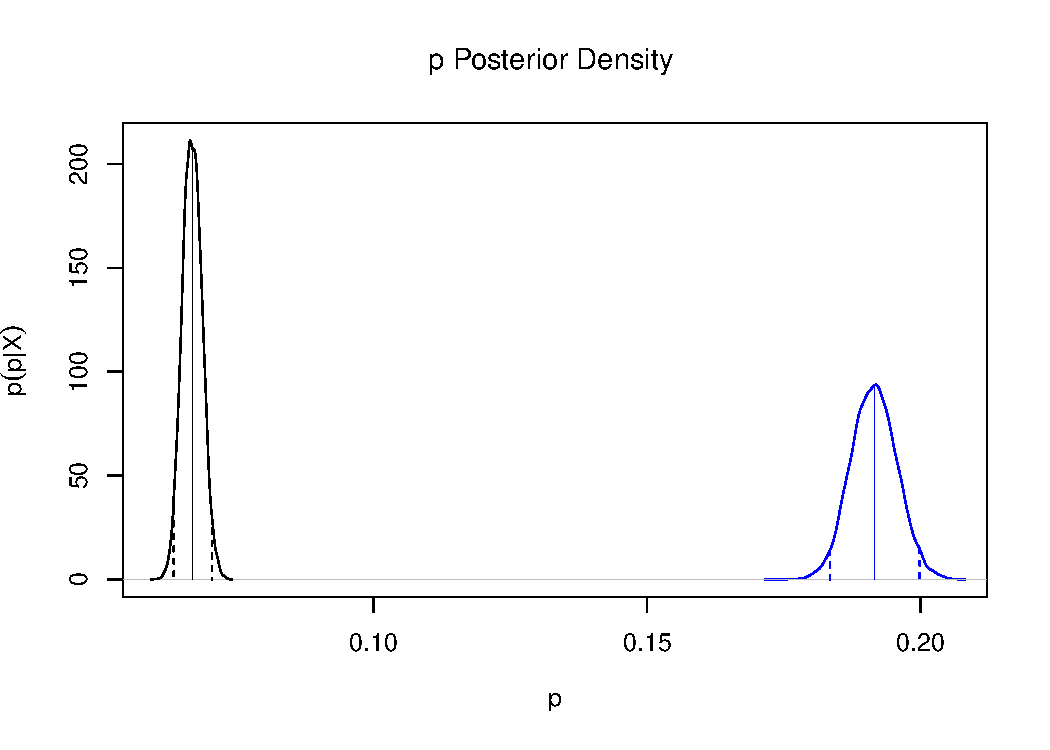
\includegraphics[width=.65\textwidth]{figure/NB_Density.pdf}
\caption{Posterior density plots (Negative Binomial model) for flood parameters (in blue), and tornado parameters (black). The solid line represents the median and the dashed lines indicate the 95\% confidence interval.}
\label{f:nbdensity}
\end{figure}
	\end{frame}
	\section{Zero Inflated Poisson Model}
	\begin{frame}
		\frametitle{Zero Inflated Poisson Model}
		The zero inflated Poisson model has two parameters p, the probability of a structural zero, and $\lambda$, the usual Poisson parameter. 
		For a single X, the probability density is:
		$$pI_{X=0}(X) + (1-p)\frac{\lambda^Xe^-\lambda}{X!}$$
	\end{frame}
	\begin{frame}
		\frametitle{Zero Inflated Poisson Model}
		One way to write the likelihood is as follows:
		$$\prod_{x_i=0}\bigg[p+(1-p)\frac{e^{-\lambda}\lambda^{x_i}}{x_i!}\bigg]\prod_{x_i \ne 0}\bigg[(1-p)\frac{e^{-\lambda}\lambda^{x_i}}{x_i!}\bigg]$$
		Bayarri, Berger, and Datta (2008)\footnotemark suggest using the prior distribution $\pi(\lambda, p) \propto \frac{1}{\sqrt{\lambda}}I(0<p<1)$. This gives us the following posterior:
		$$\prod_{x_i=0}\bigg[p+(1-p)\frac{e^{-\lambda}\lambda^{x_i}}{x_i!}\bigg]\prod_{x_i \ne 0}\bigg[(1-p)\frac{e^{-\lambda}\lambda^{x_i}}{x_i!}\bigg]\lambda^{-1/2}$$
		\footnotetext[1]{Bayarri, M., Berger, J., Datta, G. (2008). Objective testing of Poisson versus inflated Poisson models. IMS 	Collections, 3, 105-121.}
	\end{frame}
	\begin{frame}
		\frametitle{Zero Inflated Poisson Model}
		We can simplify a bit to get the following conditionals:
		\[
p(\lambda|X, p) \propto \prod_{x_i=0}\bigg[p+(1-p)\frac{e^{-\lambda}\lambda^{x_i}}{x_i!}\bigg]\prod_{x_i \ne 0}\bigg[e^{-\lambda}\lambda^{x_i}\bigg]\lambda^{-1/2}
\]

\[
p(p|X, \lambda) \propto \prod_{x_i=0}\bigg[p+(1-p)\frac{e^{-\lambda}\lambda^{x_i}}{x_i!}\bigg]\prod_{x_i \ne 0}\bigg[(1-p)\bigg]
\]

These are unrecognizable. I ended up alternatively sampling from the two using Metropolis Hastings. For lambda I settled on a gamma proposal, and for p I settled on a Beta proposal. 
	\end{frame}
	\begin{frame}
		\frametitle{Zero Inflated Poisson Model}
		Convergence of parameters (flood model):
		\centering
		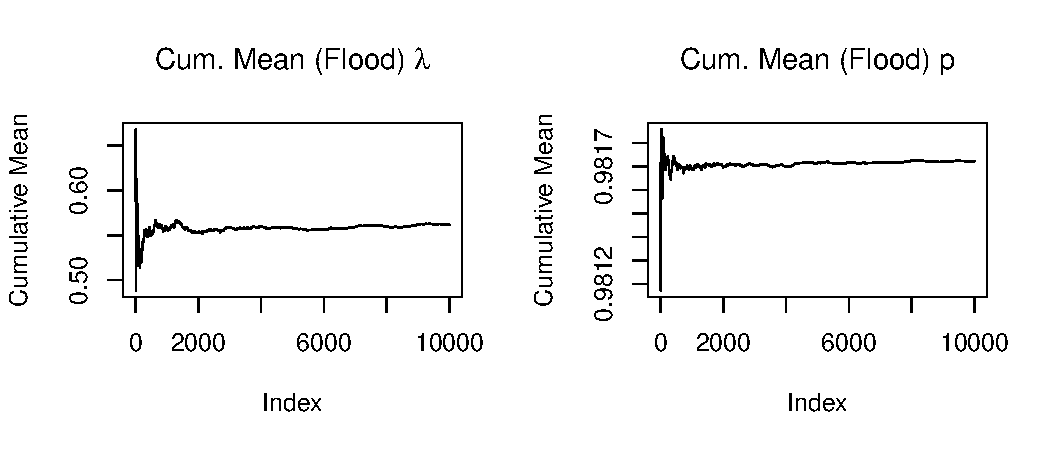
\includegraphics[width=.9\textwidth]{figure/ZIP_Flood_Conv.pdf} 
	\end{frame}
	\begin{frame}
		\frametitle{Zero Inflated Poisson Model}
		\begin{table}
    \centering
    \caption{After taking 20,000 samples from each variable and discarding 10,000 as a burn-in, we obtained the following (values are the mean of the posterior sample followed by 95 percent credible interval in parentheses)}
    \label{t:rZIP}
    \begin{tabular}{| l | l | l |}
    \hline
    Event Type & $\lambda$ & p  \\ \hline
    Tornado & 1.872 (1.030, 3.710) & 0.971 (0.968, 0.973) \\ \hline
    Flash Flood & 0.562 (0.293, 0.972) & 0.982 (0.981, 0.983) \\ \hline
    \end{tabular}
\end{table}
	\end{frame}
	\begin{frame}
		\frametitle{Zero Inflated Poisson Model}
		Posterior Densities (Blue = Flood; Black = Tornado):
		\centering
		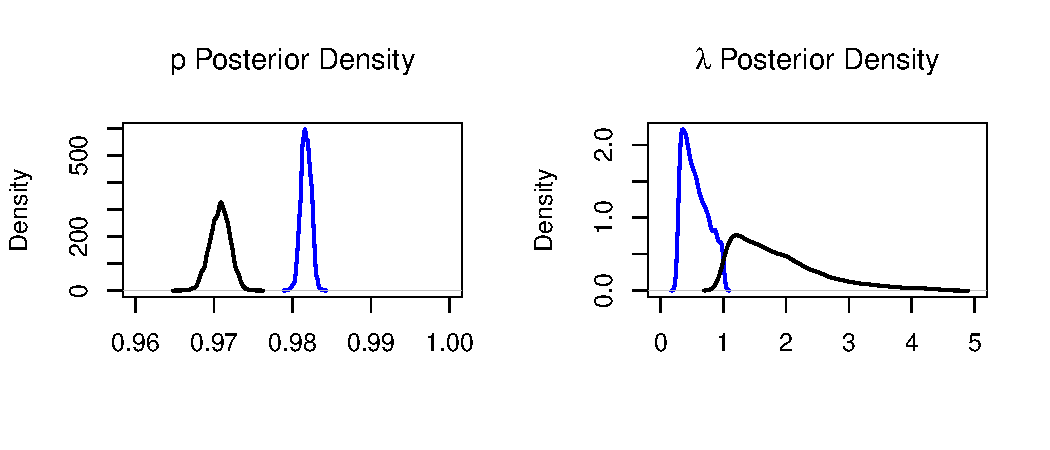
\includegraphics[width=.9\textwidth]{figure/ZIP_Density.pdf} 
	\end{frame}	
	\section{Zero Inflated Negative Binomial Model}
	\begin{frame}
		\frametitle{Zero Inflated Negative Binomial Model}
		The Zero Inflated Negative Binomial (ZINB) model has three parameters $\sigma,$ the probability of a structural zero, and $p,r$ the usual negative binomial parameters. 
		For a single $X$ the probability density is: 
		$$p(X|\sigma, p, r) = \sigma I_{X=0}(X) + (1-\sigma)\frac{\Gamma(r+X)}{\Gamma(r)X!}p^X(1-p)^r$$
	\end{frame}
	\begin{frame}
		\frametitle{Zero Inflated Negative Binomial Model}
		We took the uniform priors on $\sigma$ and $p$ and the non-informative prior $r^{-1/2}$ on $r$.
		This gave a posterior of:
		\scriptsize$$p(r,\sigma, p|X)\propto\left(\sigma + (1-\sigma)(1-p)^r\right)^Z(1-\sigma)^{N-Z}(1-p)^{(N-Z)r}p^{\sum_{i=1}^NX_i}\prod_{i=1}^N\left(\frac{\Gamma(r+X_i)}{r^{1/2}\Gamma(r)}\right)$$
		\normalsize This factors into nothing. Therefore we used the Metropolis Hastings Algorithm with proposal distributions of truncated normals.
	\end{frame}
	\begin{frame}
		\frametitle{Zero Inflated Negative Binomial Model:Results}
			$2030000$ samples were drawn for each model, with a burn in of $30000$ and one of every $250$ samples was retained, resulting in a final sample size of $8000$.
		\begin{itemize}
			\item Curse of Dimensionality; very slow convergence.
			\item High autocorrelation
			\item Low confidence in results
		\end{itemize}
		\begin{table}
			\centering
			\scalebox{.6}{
			\begin{tabular}{lcccccc}
				\toprule
				&\multicolumn{3}{c}{Flash Flood}&\multicolumn{3}{c}{Tornado}\\
				\cmidrule(r){2-4}\cmidrule(l){5-7}
				Parameter & Mean Value &Median Value & (95\% CI)& Mean Value &Median Value & (95\% CI)\\
				\midrule
				$\sigma$ & 0.308 &
				0.287&
				(0.012, 
				0.715)&
				0.29 &
				0.262&
				(0.012, 
				0.693)\\
				$p$ &  0.555 &
				0.555&
				(0.518, 
				0.591)&
				0.863 &
				0.863&
				(0.842, 
				0.882)\\
				$r$ &  0.024 &
				0.02&
				(0.014, 
				0.053)&
				0.015 &
				0.013&
				(0.009, 
				0.031)\\
				\bottomrule
			\end{tabular}}
		\end{table}
	\end{frame}
	\begin{frame}
		\frametitle{Zero Inflated Negative Binomial Model}
		\begin{figure}[p]
			\centering
			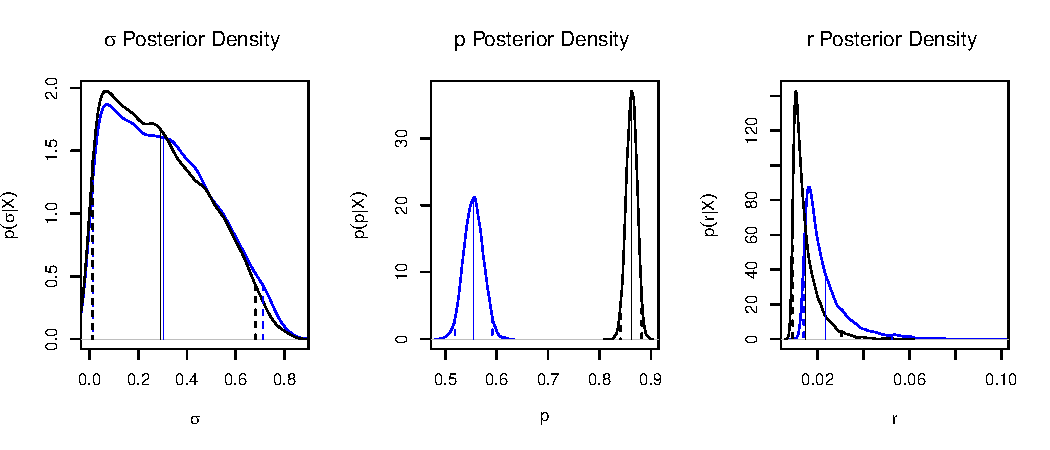
\includegraphics[width=.8\textwidth]{figure/zinbdensity-1} 
		\end{figure} 
		\begin{itemize}
			\item{$p$ can be understood to be ``dangerousness''}
			\item{$r$ can be thought of as ``duration''}
		\end{itemize}
		In this light results make sense: floods are longer lasting (on average) than tornadoes, but less dangerous (on average).
	\end{frame}
	
	\section{Conclusions}
	\begin{frame}
		\frametitle{Conclusions: Model Evaluation Table}
		% Waic dic table goes here
\begin{table}
	\centering
	\label{t:evalresults}
	\begin{tabular}{lrr}
		\toprule
		Model & DIC Flash Flood & DIC Tornado\\
		\midrule
		Poisson & 14237 & 17606\\
		Negative Binomial & 101548 & 26372\\
		ZIP & 10454 & 8727 \\
		ZINB & 10804&7166\\
		\bottomrule
	\end{tabular}
\end{table}

The Zero Inflated Poisson model has the lowest DIC, for Flash Floods and the ZINB has the lowest for Tornadoes. For estimating or predicting lethality counts for weather it appears that Zero inflated models out perform their plain variants however, which zero inflated model is not clear, as we only did two weather events and the ZINB and ZIP were similar.
	\end{frame}
	\begin{frame}
	
		\frametitle{Conclusions: Future Work}
		% List of things we might have done if we'd had time
		\begin{enumerate}
			\item{Re-parameterize the ZINB model/look into other techniques to improve convergence.}
			\item{See if the results hold on other extreme weather events.}
		\end{enumerate}
	\end{frame}
	\begin{frame}
		\frametitle{Conclusions}
		Questions?
	\end{frame}
\end{document} 